\newpage\section{Information theory}

%%%%%%%%%%%%%%%%%%%%%%%%%%%%%%%%%%%%%%%%%%%%%%%%%%%%%%%%%%%%%%%%%%%%%%%%%%%%%%%%
\subsection{Self-information (information content)}
%%%%%%%%%%%%%%%%%%%%%%%%%%%%%%%%%%%%%%%%%%%%%%%%%%%%%%%%%%%%%%%%%%%%%%%%%%%%%%%%

The self-information (a.k.a. \textit{information content},~\textit{surprisal},
or \textit{Shannon information}) is a quantity used in information theory which
is derived from the probability of a certain event occurring from a random
variable. The self-information was defined by Claude Shannon~\cite{} such that
the following axioms were met:

\begin{enumerate}
    \item An event that is 100\% probable is perfectly unsurprising and
    therefore yields no information content.
    \item The less probable an event is, the more surprising, and therefore the
    more information it yields.
    \item The total information of independently measured events, is the
    sum of their respective self-information.
\end{enumerate}

\begin{equation}
    I(x):=-\log_b(p(x))
\end{equation}

\cite{ElementaryInformationTheory1979}

%%%%%%%%%%%%%%%%%%%%%%%%%%%%%%%%%%%%%%%%%%%%%%%%%%%%%%%%%%%%%%%%%%%%%%%%%%%%%%%%
\subsection{Entropy (average information)}
%%%%%%%%%%%%%%%%%%%%%%%%%%%%%%%%%%%%%%%%%%%%%%%%%%%%%%%%%%%%%%%%%%%%%%%%%%%%%%%%

Claude Shannon argued

\begin{equation}
    H(x)=\gls{E}\;[I(x)]
\end{equation}

%%%%%%%%%%%%%%%%%%%%%%%%%%%%%%%%%%%%%%%%%%%%%%%%%%%%%%%%%%%%%%%%%%%%%%%%%%%%%%%%
\newpage\subsection{Kullback-Leibler divergence (information gain)\label{sec:kl_div}}
%%%%%%%%%%%%%%%%%%%%%%%%%%%%%%%%%%%%%%%%%%%%%%%%%%%%%%%%%%%%%%%%%%%%%%%%%%%%%%%%

The Kullback-Leibler divergence (a.k.a. \textit{relative entropy} and
\textit{I-divergence}) a measure of how one probability distribution $P$ differs
from another, $Q$. For the distributions $P$ and $Q$ for a continuous random
variable, the relative entropy integral is:

\begin{equation}
    D_{KL}(P\;||\;Q) = \int_{-\infty}^{\infty}p(x)\log(\frac{p(x)}{q(x)})\;dx.
    \label{eq:kullback-leibler}
\end{equation}

Note that $D_{KL}(P\;||\;Q)$ is only finite if the support set of $P$ is
contained in the support set of $Q$~\cite[p.~251]{Cover2006}. In the context
of Bayesian inference $D_{KL}(P\;||\;Q)$, read as \textit{the KL-divergence of P
given Q}, is a measure of the information gained by revisiting one's beliefs
from a prior probability distribution $Q$ to a posterior probability
distribution $P$. For example the $D_{KL}(P\;||\;Q)$ for
$P\sim{}\mathcal{N}(\mu_1,\sigma_1)$ and $Q\sim{}\mathcal{N}(\mu_2,\sigma_2)$ can be derived
analytically (\autoref{app:norm_kl}) to be:

\begin{equation}
    D_{KL}(P\;||\;Q) = \log\frac{\sigma_2}{\sigma_1} + \frac{\sigma_1^2 + (\mu_1-\mu_2)^2}{2\sigma_2^2} - \frac{1}{2}.
\end{equation}
%\begin{equation}
%
%\end{equation}

One noteworthy characteristic of the KL-divergence is its asymmetry, that is
$D_{KL}(P\;||\;Q)\neq{}D_{KL}(Q\;||\;P)$. This means that KL-divergence makes
for a poor \textit{distance} metric as is commonly done with, for example,
squared-errors. This may at first present KL-divergence as a suboptimal choice
as a general metric, however when considering the relation between the posterior
and the priori, the relative information gain when travelling from one to the
other \textbf{is} inherently asymmetric by their very nature. For example, for
the case of

\begin{figure}[!htp]
    \centering
    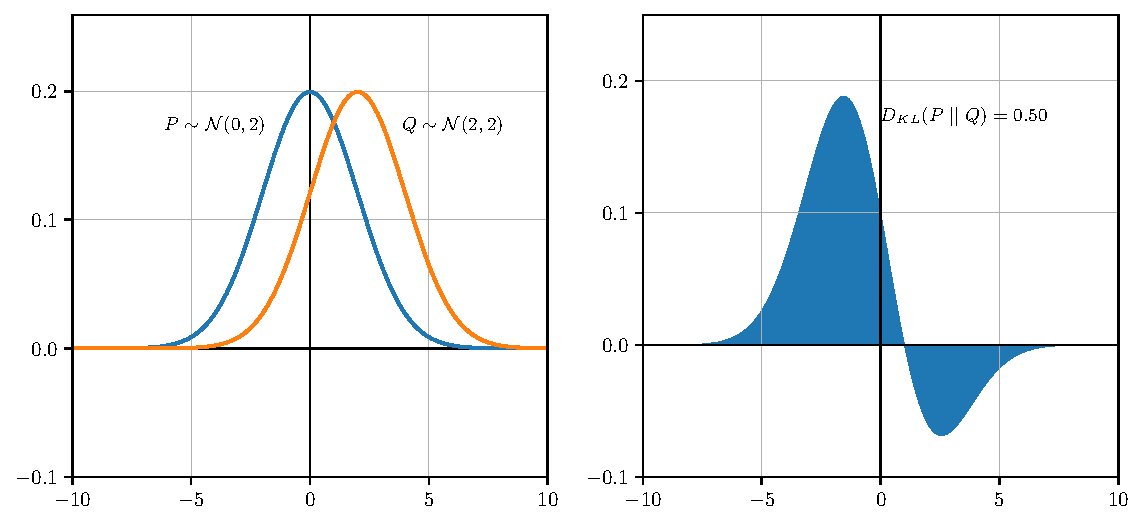
\includegraphics[width=0.9\linewidth]{graphics/kullback-leibler.pdf}
    \caption{\textbf{Kullback-Leibler example} for the distributions of
    $P\sim{}\mathcal{N}(0,2)$ and $Q\sim{}\mathcal{N}(2,2)$. }
    \label{fig:kullback-leibler}
\end{figure}

%%%%%%%%%%%%%%%%%%%%%%%%%%%%%%%%%%%%%%%%%%%%%%%%%%%%%%%%%%%%%%%%%%%%%%%%%%%%%%%%
\newpage\subsection{Jensen-Shannon divergence (information radius)}
%%%%%%%%%%%%%%%%%%%%%%%%%%%%%%%%%%%%%%%%%%%%%%%%%%%%%%%%%%%%%%%%%%%%%%%%%%%%%%%%

The Jensen-Shannon divergence (a.k.a. \textit{information radius} and
\textit{total divergence to the average}) is based on the KL-divergence
(\autoref{sec:kl_div}), however it has been extended with the differences that
it is symmetric, and always has a finite value~\cite{Endres2003, Fuglede2004}.


\begin{equation}
    \begin{aligned}
    D_{JS}(P\;||\;Q) &= \frac{1}{2}D_{KL}(P\;||\;M) + \frac{1}{2}D_{KL}(Q\;||\;M)
    \end{aligned}
\end{equation}
\begin{equation*}
    \text{where}\;\;
    \begin{aligned}
        M = \frac{1}{2}(P+Q)
    \end{aligned}
\end{equation*}